\documentclass[tikz,border=12pt]{standalone}
\usepackage[T1]{fontenc}
\usepackage{mathpazo}
\usepackage{amsmath,amssymb}
\usetikzlibrary{arrows.meta, positioning, calc, decorations.pathreplacing}

\definecolor{stblue}{HTML}{7B97AD}
\definecolor{rwgold}{HTML}{B8995E}
\definecolor{sage}{HTML}{7A9A7E}
\definecolor{dkbrown}{HTML}{3D3530}
\definecolor{wmgray}{HTML}{7B7067}
\definecolor{cream}{HTML}{F9F6F0}
\definecolor{border}{HTML}{D4C9B8}
\definecolor{terracotta}{HTML}{C47A6A}
\definecolor{lavender}{HTML}{907EA0}

\begin{document}
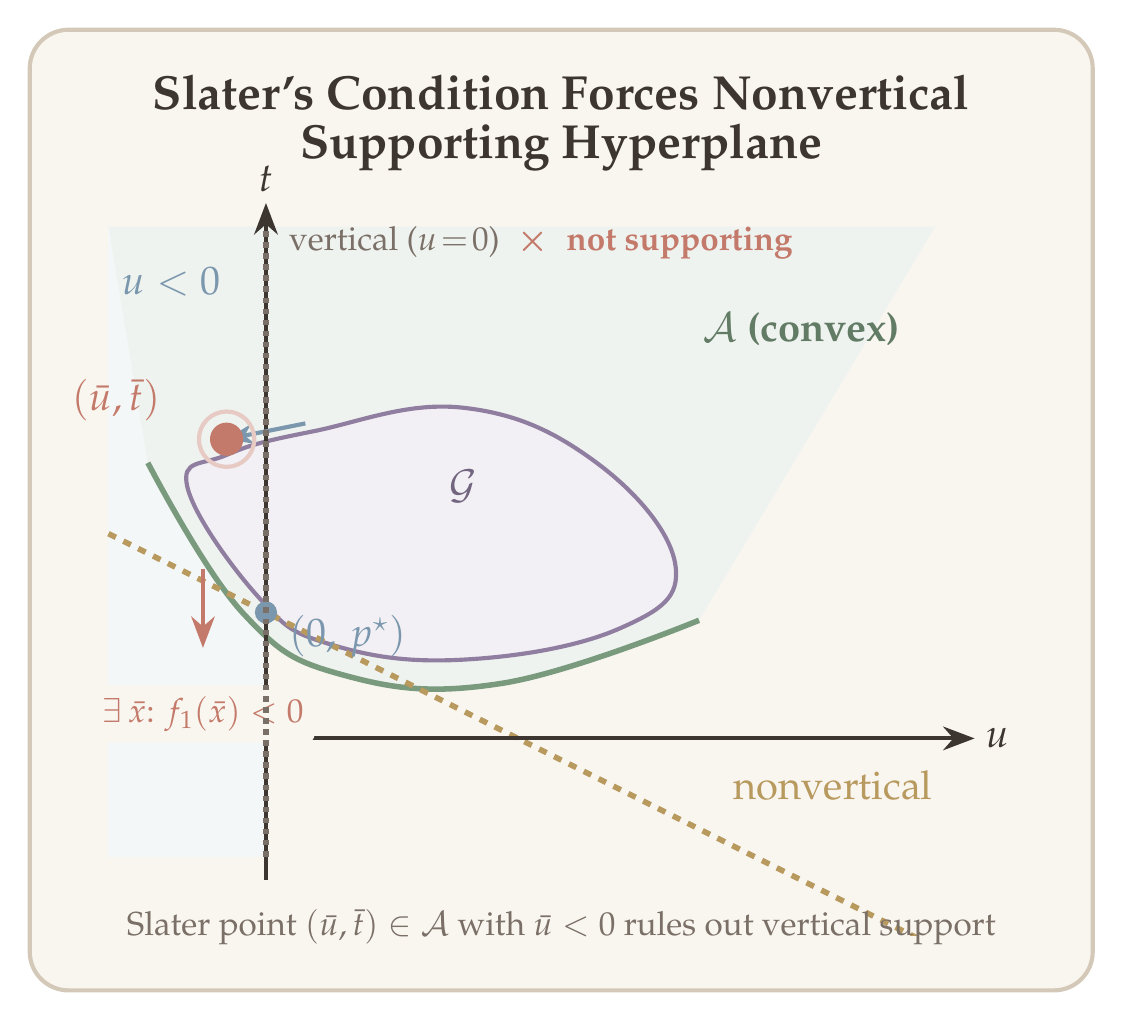
\begin{tikzpicture}[>={Stealth[length=4mm, width=3mm]}, line width=1.5pt]

% Background
\fill[cream, rounded corners=14pt] (-3,-3.2) rectangle (10.5,9);
\draw[border, line width=1.5pt, rounded corners=14pt] (-3,-3.2) rectangle (10.5,9);

% Title
\node[font=\LARGE\bfseries, text=dkbrown, align=center] at (3.75,8.2)
  {Slater's Condition Forces Nonvertical};
\node[font=\LARGE\bfseries, text=dkbrown, align=center] at (3.75,7.5)
  {Supporting Hyperplane};

% --- Fills and shapes (drawn BEFORE axes) ---

% Highlight the u<0 region
\fill[stblue!8] (-2,-1.5) rectangle (0,6.5);

% Epigraph set A (convex)
\begin{scope}
\clip (-2,-1.5) rectangle (8.5,6.5);
\fill[sage!12]
  plot[smooth, tension=0.7] coordinates {
    (-1.5,3.5) (-0.3,1.6) (1,0.8) (3,0.7) (5.5,1.5)
  } -- (8.5,6.5) -- (-2,6.5) -- cycle;
\draw[sage, line width=2pt]
  plot[smooth, tension=0.7] coordinates {
    (-1.5,3.5) (-0.3,1.6) (1,0.8) (3,0.7) (5.5,1.5)
  };
\end{scope}

% The set G (smaller blob inside A)
\fill[lavender!12, draw=lavender, line width=1.5pt]
  plot[smooth cycle, tension=0.7] coordinates {
    (-1,3.2) (-0.1,1.8) (0.8,1.2) (2.5,1.0)
    (4.5,1.4) (5.2,2.2) (4.2,3.5)
    (2.5,4.2) (0.6,3.9) (-0.5,3.6)
  };

% Nonvertical supporting hyperplane (clipped to canvas)
\begin{scope}
\clip (-2.5,-2.5) rectangle (9,7);
\draw[rwgold, line width=2pt, dashed]
  (-2, {1.6+0.5*2}) -- (8.5, {1.6-0.5*8.5});
\end{scope}

% --- Axes (drawn AFTER fills so they remain visible) ---
\draw[->, dkbrown, line width=1.5pt] (-2,0) -- (9,0)
  node[right, font=\Large, text=dkbrown] {$u$};
\draw[->, dkbrown, line width=1.5pt] (0,-1.8) -- (0,6.8)
  node[above, font=\Large, text=dkbrown] {$t$};

% --- Labels and annotations ---

% Arrows showing that A extends past u=0 into the u<0 region
\draw[stblue, line width=1.5pt, ->, >=Stealth] (0.5,4.0) -- (-0.5,3.8);
\node[font=\Large\bfseries, text=stblue] at (-1.2,5.8) {$u < 0$};

\node[font=\Large\bfseries, text=sage!80!black] at (6.8,5.2) {$\mathcal{A}$ (convex)};
\node[font=\Large\bfseries, text=lavender!80!black] at (2.5,3.2) {$\mathcal{G}$};

% Slater point (strictly feasible: u < 0, clearly in INTERIOR of A)
\draw[terracotta!40, line width=1.5pt] (-0.5,3.8) circle (10pt);
\fill[terracotta] (-0.5,3.8) circle (6pt);
\node[font=\Large\bfseries, text=terracotta, anchor=east] at (-1.2,4.3) {$(\bar{u}, \bar{t})$};

% Annotation showing Slater condition near the point
\node[font=\large, text=terracotta, align=left, fill=cream, inner sep=4pt,
      rounded corners=3pt, anchor=north] at (-0.8,0.7)
  {$\exists\, \bar{x}$: $f_1(\bar{x}) < 0$};

% p* at u=0
\fill[stblue] (0,1.6) circle (4pt);
\node[font=\Large\bfseries, text=stblue, right] at (0.15,1.3) {$(0,\, p^\star)$};

\node[font=\Large, text=rwgold] at (7.2,-0.6) {nonvertical};

% Vertical line at u=0 (not supporting because A extends past it)
\draw[wmgray, line width=2pt, dotted]
  (0,-1.5) -- (0,6.5);
\node[font=\large, text=wmgray, right, align=left] at (0.15,6.3) {vertical ($u\!=\!0$)\; \textcolor{terracotta}{\bfseries$\boldsymbol{\times}$\; not supporting}};

% Arrow from Slater point to show it's in u<0 region
\draw[terracotta, line width=1.2pt, ->] (-0.8,2.15) -- (-0.8,1.15);

% Legend annotation
\node[font=\large, text=wmgray, align=center] at (3.75,-2.4)
  {Slater point $(\bar{u}, \bar{t}) \in \mathcal{A}$ with $\bar{u} < 0$ rules out vertical support};

\end{tikzpicture}
\end{document}
